\documentclass[10 pt,usenames,dvipsnames, oneside]{article}
\usepackage{../../../modelo-ensino-medio}



\begin{document}

\begin{center}
  \begin{minipage}[l]{3cm}
\includegraphics[width=2cm]{logo}    
\end{minipage}\hfill
\begin{minipage}[r]{.8\textwidth}
 {\Large \scshape Atividade: Gráficos dos logaritmos}  
\end{minipage}
\end{center}
\vspace{.2cm}

\ifdefined\prof
%Habilidades da BNCC
\begin{objetivos}
\item \textbf{EM13MAT403} Analisar e estabelecer relações, com ou sem apoio de tecnologias digitais, entre as representações de funções exponencial e logarítmica expressas em tabelas e em plano cartesiano, para identificar as características fundamentais (domínio, imagem, crescimento) de cada função.
\end{objetivos}

%Caixa do Para o Professor
\begin{goals}
%Objetivos específicos
\begin{enumerate}
\item Reconhecer gráficos das funções logarítmicas de bases maior do que $1$ e menor do que $1$.
\item Relacionar os gráficos de funções logarítmicas de base a $a>1$ e $\frac{1}{a}$.
\end{enumerate}

\tcblower

%Orientações e sugestões
\begin{itemize}
\item 	O enunciado apresenta os valores dos logaritmos para encurtar o tempo da atividade, tendo em vista que cálculos de logaritmos já foram explorados nas atividades anteriores. Recomenda-se a reflexão sobre os valores do logaritmo de base $1/2$, se necessário com mediação do/a  professor/a, para que se conclua que eles são iguais a "menos"\, os valores listados. Como mediação pode-se comparar $2^3=8$, $2^{-3}=1/8$, $1/2^3=1/8$ e $(1/2)^{-3}=8$.
\end{itemize}
\end{goals}

\bigskip
\begin{center}
{\large \scshape Atividade}
\end{center}
\fi

Utilize as aproximações abaixo, com dois dígitos de precisão, dos logaritmos em base $2$ para esboçar o gráfico de $f(x) = \log_{2} x$ no espaço quadriculado abaixo.
\begin{align*}
& \log_{2} 1/8 = -3; \,\, \log_{2} 1/4 = -2; \,\, \log_{2} 1/2 = -1; \,\, \log_{2} 1 = 0; \,\, \log_{2} 2  = 1; \,\, \log_{2} 3  =  1{,}58; \,\,\\
& \log_{2} 4  = 2; \,\, \log_{2} 5 = 2{,}32; \,\, \log_{10} 1 = 0; \,\, \log_{2} 6 = 2{,}58; \,\, \log_{2} 7  = 2{,}8; \,\, \log_{2} 8  = 3; \,\,\\
& \log_{2} 9  = 3{,}16; \,\, \log_{2} 10  = 3{,}32.
\end{align*}
Após esboçar esse gráfico, converse com seus colegas e com o professor como utilizar esses valores para esboçar o gráfico $g(x) = \log_{1/2} x$ e tente traçá-lo.

\begin{figure}[H]
\centering

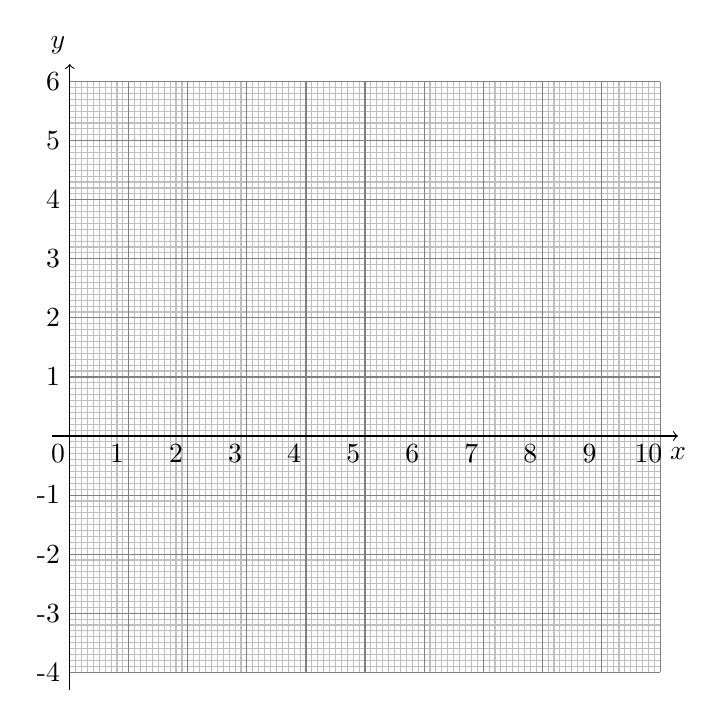
\begin{tikzpicture}[scale=.75]
\foreach \i in {0,...,100}{% 10 (instead of 9) is used here to make sure the last line is drawn.
            \draw[lightgray] (0.1*\i,0) -- (0.1*\i,10);
            \draw[lightgray] (0,0.1*\i) -- (10,0.1*\i);}
\foreach \n in {0,...,10}{% 10 (instead of 9) is used here to make sure the last line is drawn.
            \draw[gray] (\n,0) -- (\n,10);
            \draw[gray] (0,\n) -- (10,\n);
            \node at (\n-0.2, 3.7) {\n};}

	\foreach \n in {-4,...,-1,1,2,...,6}{\node[left] at (0, \n+4) {\n};}
\draw[black,->] (0,-0.3) -- (0,10.3);
\node[black, above] at (-0.2,10.3) {$y$};
\draw[black,->] (-0.3,4.0) -- (10.3,4.0);
\node[black] at (10.3,3.7) {$x$};
\end{tikzpicture}
\end{figure}

\ifdefined\prof
\begin{solucao}

	Os gráficos de $f$ em verde e $g$ em laranja.

	\begin{figure}[H]
	\centering

	\begin{tikzpicture}[scale=.75]
	\foreach \n in {0,...,10}{% 10 (instead of 9) is used here to make sure the last line is drawn.
	            \draw[gray] (\n,0) -- (\n,10);
	            \draw[gray] (0,\n) -- (10,\n);}
	%            \node at (\n-0.2, 3.7) {\n};
	\node [below left] at (0,4) {0};
	\foreach \n in {-4,...,-1,1,2,...,6}{\node[left] at (0, \n+4) {\n};}
	\draw[black,->] (0,-0.3) -- (0,10.3);
	%\node[black] at (-0.2,10.3) {y};
	\draw[black,->] (-0.3,4.0) -- (10.3,4.0);
	%\node[black] at (10.3,3.7) {x};
	\draw[primario!80, domain=0.125:10,samples=1000, thick] plot (\x, {4+log2(\x)});
	\draw[\currentcolor!80, domain=0.125:10,samples=1000, thick] plot (\x, {4-log2(\x)});
	\draw[black,->] (-0.3,4.0) -- (10.3,4.0);
	\node[black] at (10.3,3.7) {$x$};
	\node[black, above] at (-0.2,10.3) {$y$};
	\end{tikzpicture}
	\end{figure}

\end{solucao}
\fi

\end{document}